\chapter{Coil array WPT}\chaplab{result}
% 通过上一章节的讲解,我们知道了无线传输系统在水下的基本表现。这章将介绍我们设计出的水下线圈组wpt系统,通过将大型的双线圈结构降解为多个小线圈结构,这使得内部线圈里面的磁场大幅减小,从而实现对AUV系统内部的电磁保护。
Through the explanation in the previous chapter, we know the basic performance of the wireless transmission system underwater. This chapter will introduce the underwater coil group wpt system we designed, by degrading a large double coil structure into multiple small coil structures. This greatly reduces the magnetic field in the internal coil, thereby achieving electromagnetic protection inside the AUV system.

\begin{figure}[htbp]
    \centering
    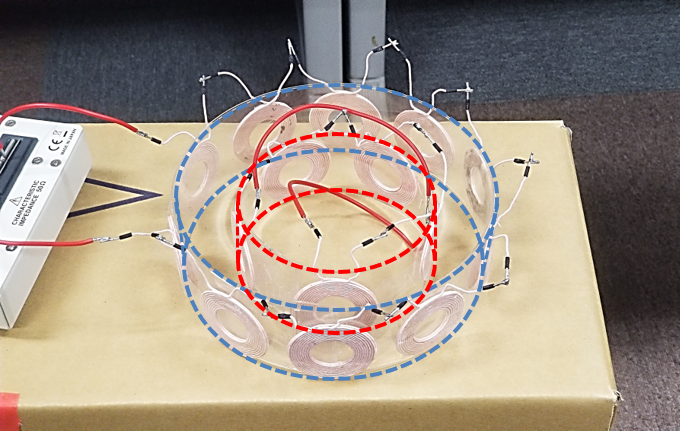
\includegraphics[width=0.7\linewidth]{images/3_coil_array_structure.png}
    \caption{Underwater sensor networks architecture.}
    \label{fig:3_coil_array_structure}
\end{figure}

% 参数表格

\begin{figure}[htbp]
    \centering
    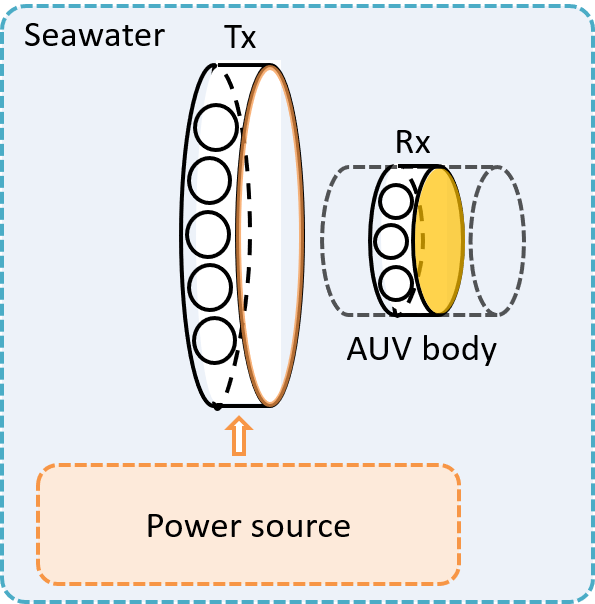
\includegraphics[width=0.5\linewidth]{images/3_coil_array_uwpt.png}
    \caption{Underwater sensor networks architecture.}
    \label{fig:3_coil_array_uwpt}
\end{figure}

% \begin{figure}[htbp]
%     \centering
%     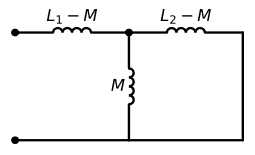
\includegraphics{images/3_mutual_inductance.png}
%     \caption{svg image}
% \end{figure}

\section{Simulation evaluation}


\begin{figure}[htbp]
    \begin{subfigure}{0.5\textwidth}
        \centering
        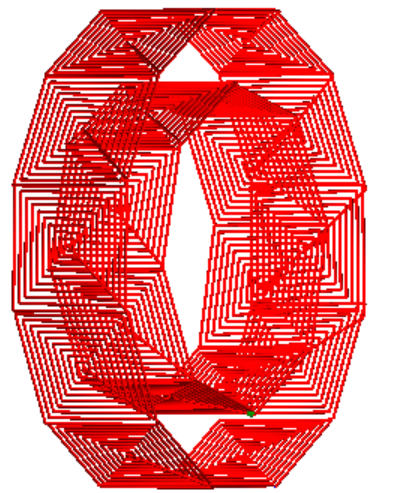
\includegraphics[height=6.4cm]{images/4_coil_array_system.png}
    \caption{Coil-array IPT structure.}
        \label{fig:subim1}
    \end{subfigure}
    \begin{subfigure}{0.5\textwidth}
        \centering
        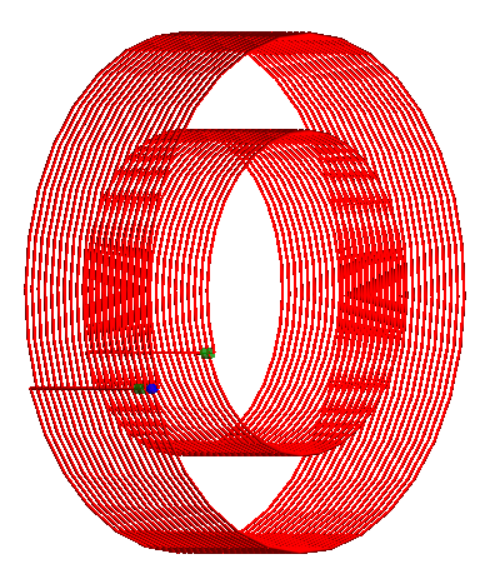
\includegraphics[height=6.4cm]{images/4_two_ring_system.png}
    \caption{Two ring IPT structure.}
        \label{fig:subim2}
    \end{subfigure}

    \caption{Two ring structure.}
    \label{fig:3_two_ring_coil}
\end{figure}


\begin{figure}[htbp]
    \centering
    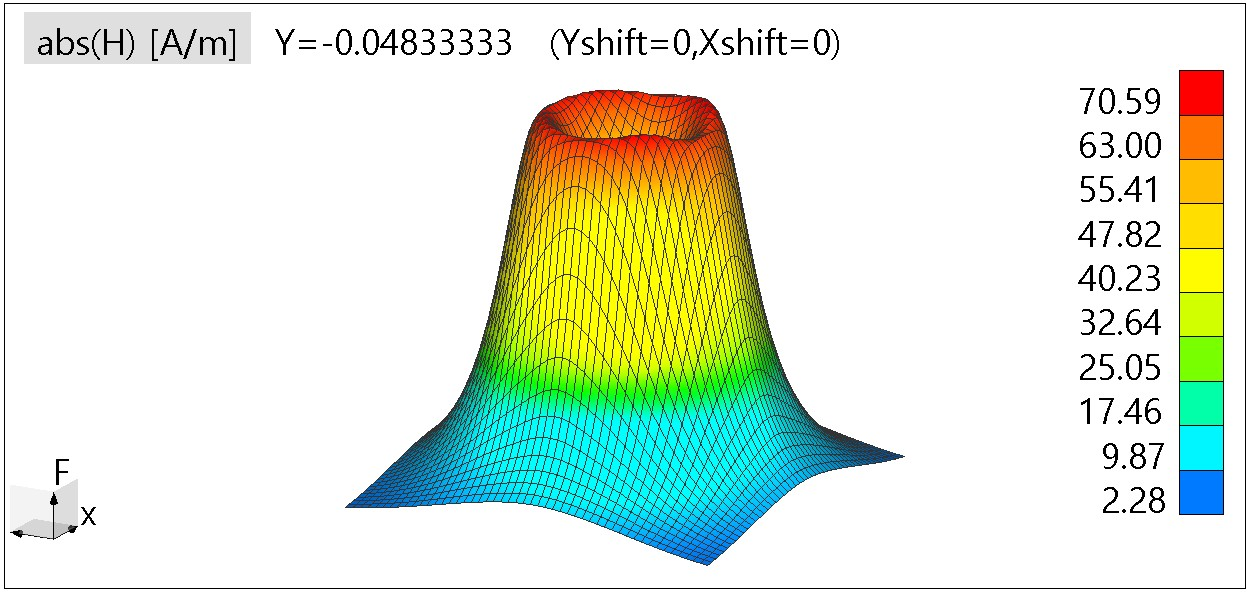
\includegraphics[width=0.9\linewidth]{images/4_coil_array_near_field_distribution.JPG}
    \caption{Coil-array IPT structure.}
\end{figure}

\begin{figure}[htbp]
    \centering
    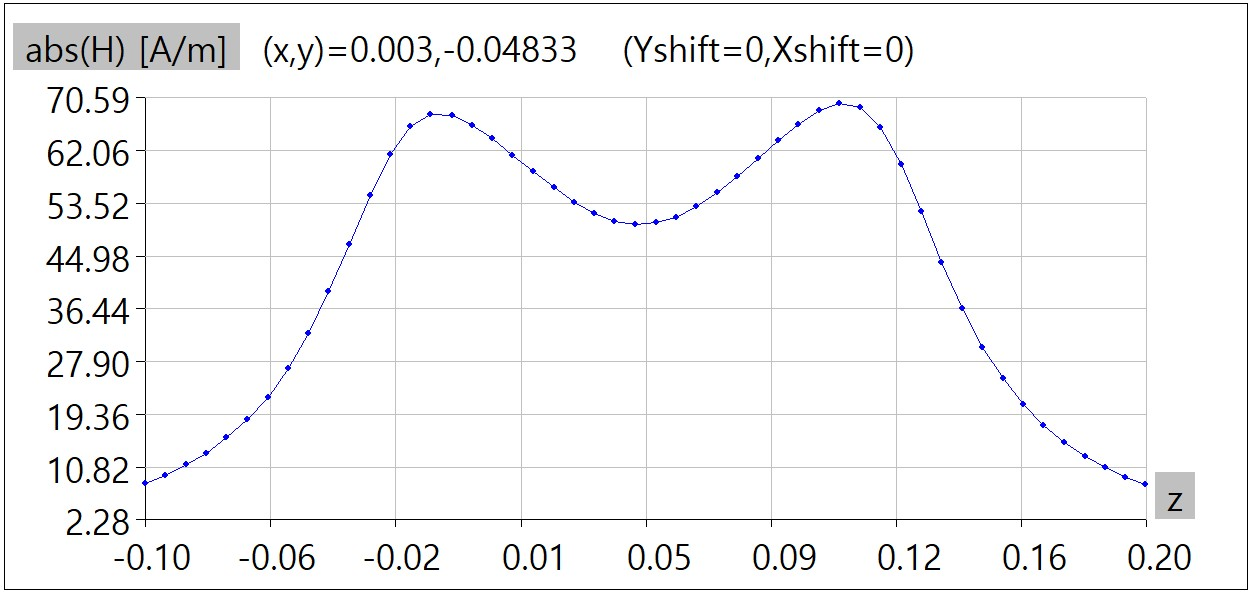
\includegraphics[width=0.9\linewidth]{images/4_coil_array_near_field_distribution_cut.JPG}
    \caption{Coil-array IPT structure.}
\end{figure}

\begin{figure}[htbp]
    \centering
    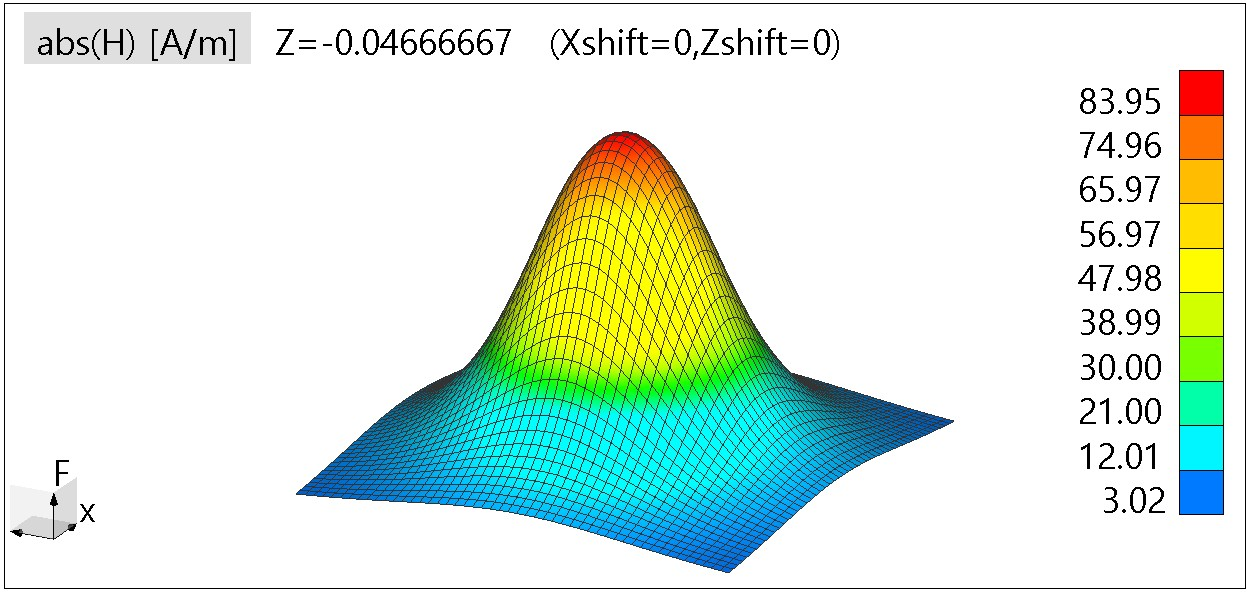
\includegraphics[width=0.9\linewidth]{images/4_two_ring_near_field_distribution.JPG}
    \caption{Coil-array IPT structure.}
\end{figure}

\begin{figure}[htbp]
    \centering
    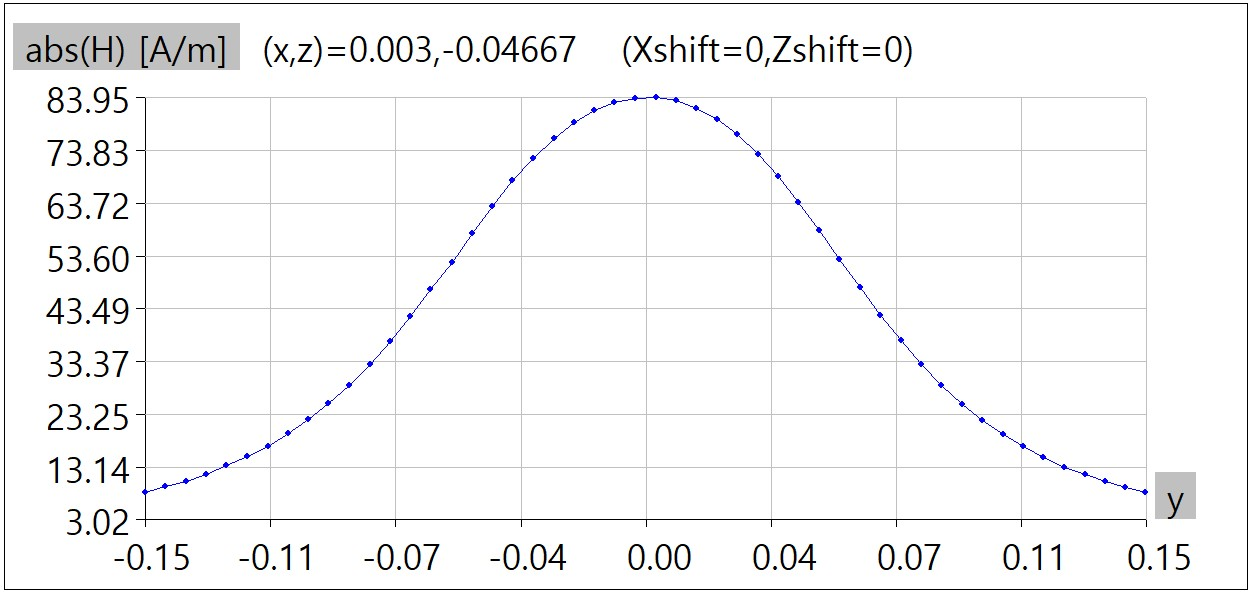
\includegraphics[width=0.9\linewidth]{images/4_two_ring_near_field_distribution_cut.JPG}
    \caption{Coil-array IPT structure.}
\end{figure}

% 改变内部线圈的偏移,双方向下的偏移。

\subsection{Simulation evaluation}


\section{Coil array WPT in the air}
\begin{figure}[htbp]
    \centering
    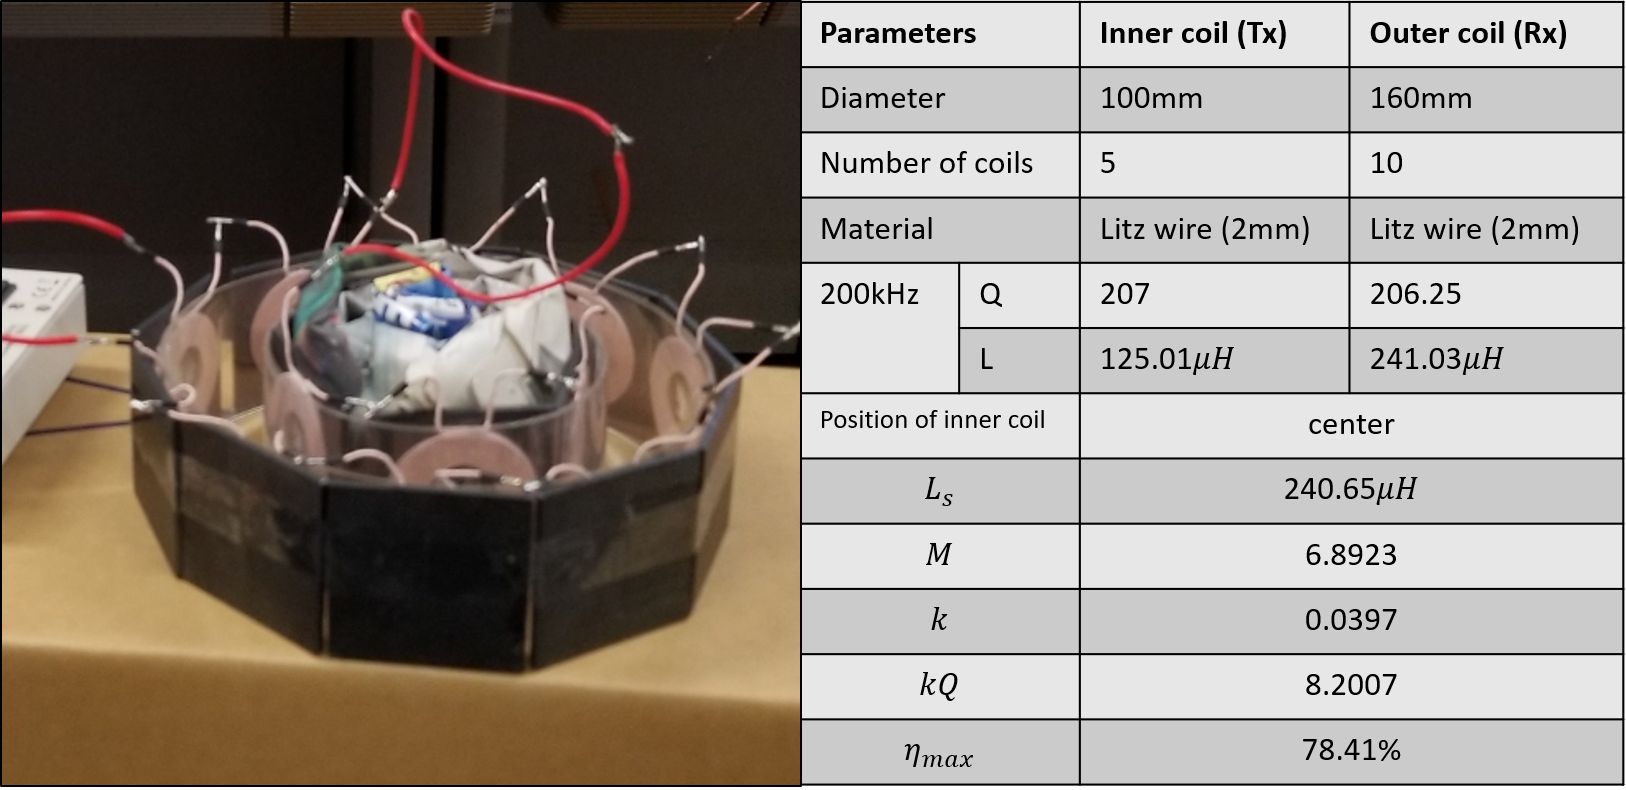
\includegraphics[width=1.0\linewidth]{images/4_coil_5_10_with_ferrite.png}
    \caption{Coil-array IPT structure.}
\end{figure}
\begin{figure}[htbp]
    \centering
    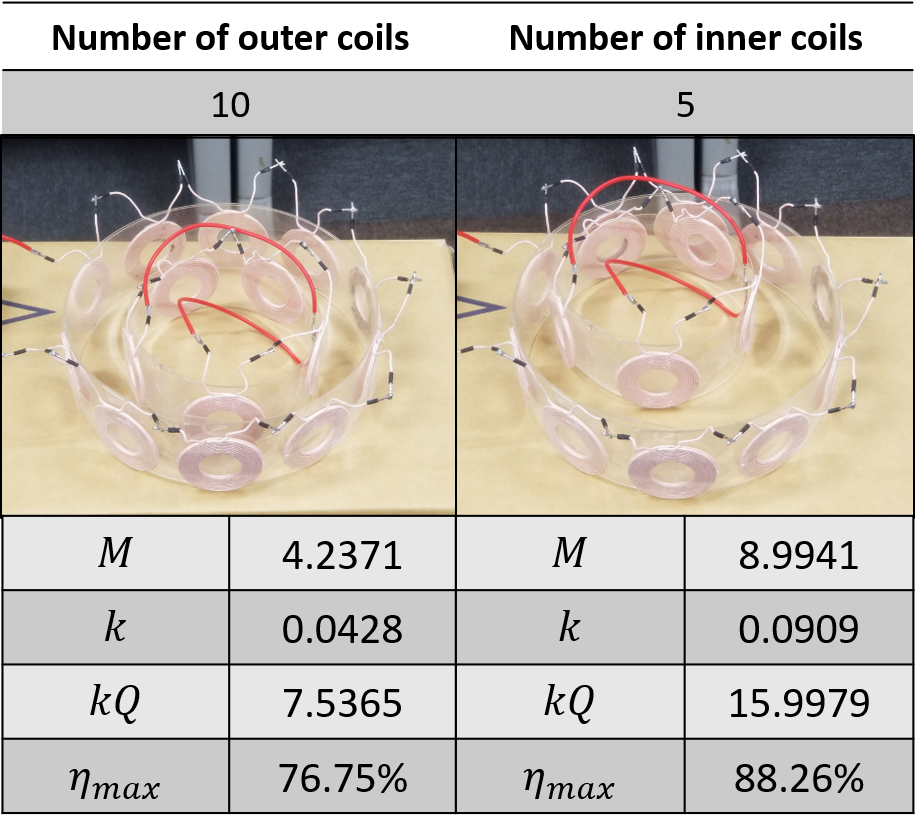
\includegraphics[width=0.6\linewidth]{images/4_coil_5_10_without_ferrite.png}
    \caption{Coil-array IPT structure.}
\end{figure}
\begin{figure}[htbp]
    \centering
    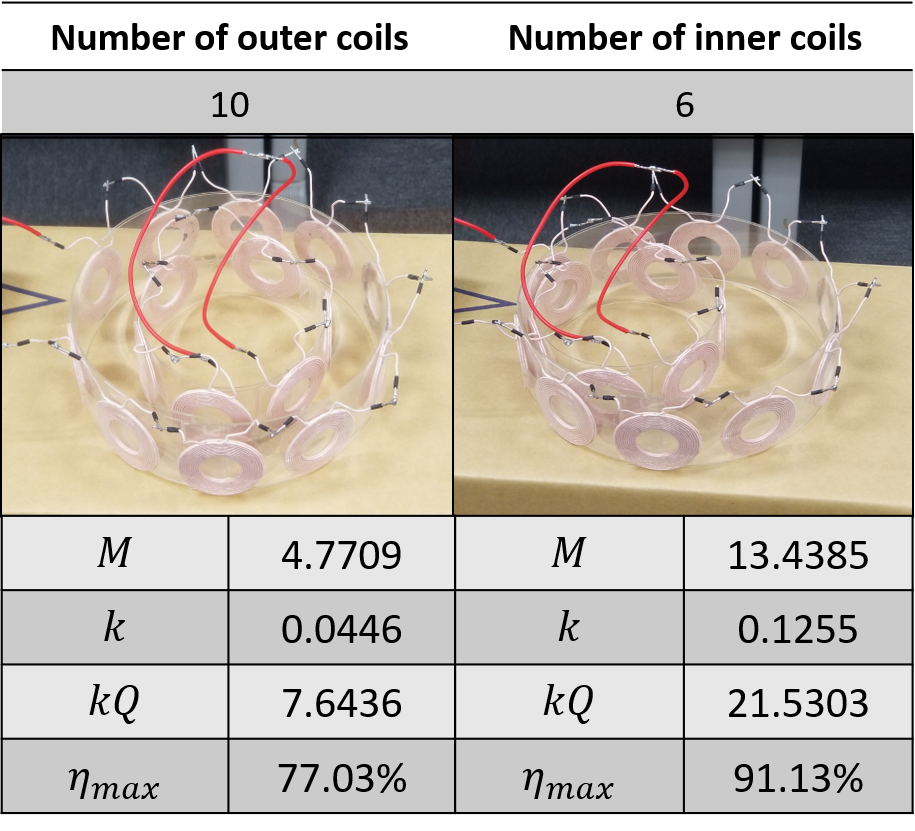
\includegraphics[width=0.6\linewidth]{images/4_coil_6_10_without_ferrite.png}
    \caption{Coil-array IPT structure.}
\end{figure}
\begin{figure}[htbp]
    \centering
    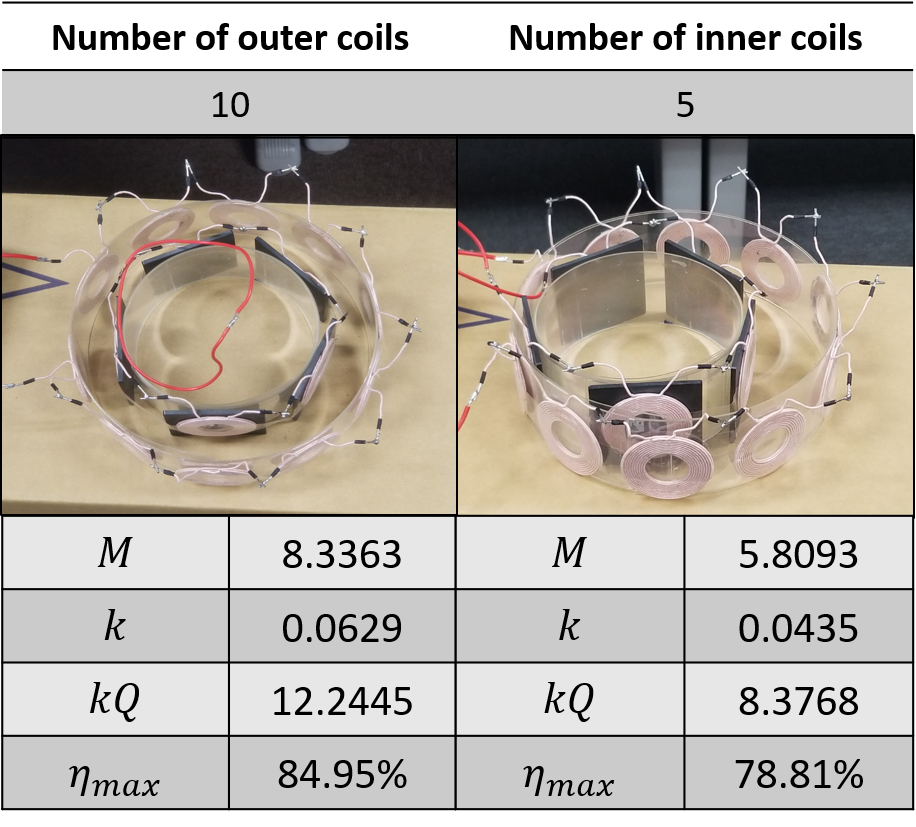
\includegraphics[width=0.6\linewidth]{images/4_coil_6_10_inner_with_ferrite.png}
    \caption{Coil-array IPT structure.}
\end{figure}

\begin{table}[htbp]
    \centering
    \caption{Maximum power transfer efficiency.}
    \begin{tabular}{|>{\centering\arraybackslash}m{3.3cm}|>{\centering\arraybackslash}m{2.5cm}|>{\centering\arraybackslash}m{2.5cm}|>{\centering\arraybackslash}m{2.5cm}|>{\centering\arraybackslash}m{2.5cm}|}
        \hline
        \textbf{Shift}                                    & \textbf{Numbers of coiL (Outer - Inner)} & \textbf{Both coils with ferrite} & \textbf{Both coils without ferrite} & \textbf{Outer coils without ferrite, inner coils with ferrite} \\ \hline
        \multirow{2}{3.3cm}{Inner coil in the center}         & 10 - 5                             & 78.41\%                          & 76.75\%                             & 84.95\%                            \\ \cline{2-5}
                                                          & 10 - 6                             &                                  & 77.03\%                             &                                    \\ \hline
        \multirow{2}{3.3cm}{Inner coil close to the one side} & 10 - 5                             &                                  & 88.26\%                             & 78.80\%                            \\ \cline{2-5}
                                                          & 10 - 6                             &                                  & 91.13\%                             &                                    \\ \hline
    \end{tabular}
\end{table}

\begin{itemize}
\item When we increase the number of inner coils, the maximum PTE (Power transfer efficiency) will increase.
\item If the numbers of outer and inner coils are the same, when outer coils without ferrite and inner coils with ferrite, we can get the maximum PTE.
\item When there is no ferrite outside the inner coil, the PTE will increase if the inner coil deviates from the middle, and vice versa.
\end{itemize}


\section{Coil array WPT under seawater}